
\subsection{Axial Shielding Factor Measurements\label{sec:axial}}

In these measurements, a witness cylinder was used as a magnetic
shield.  The shield was subjected to a low-frequency AC magnetic field
of $\sim 1$~Hz.  The amplitude of the shielded magnetic field $B_s$
was measured at the center of the witness cylinder using a fluxgate
magnetometer.  Changes in $B_s$ with temperature signify a dependence
of the permeability $\mu$ on temperature.  The relative slope of
$\mu(T)$ can then be calculated using
\begin{equation}
\frac{1}{\mu}\frac{d\mu}{dT}=-\frac{\frac{1}{B_s}\frac{dB_s}{dT}}{\frac{\mu}{B_s}\frac{dB_s}{d\mu}}.
\label{eqn:axial}
\end{equation}
The numerator was taken from the measurements described above. The
denominator was taken from finite-element simulations of the shielding
factor for this geometry as a function of $\mu$.

This measurement technique was sufficiently robust to extract the
temperature dependence of the shielding factor with some degree of
certainty. Possible drifts and temperature dependence of the fluxgate
magnetometer offset were mitigated by using an AC magnetic field.  Any
temperature coefficients in the rest of the instrumentation were
controlled by performing the same measurements with a copper
cylindrical shell with the similar size and shape as the mu-metal
witness cylinders in place of the mu-metal witness cylinder.

This technique is quite different than the usual transformer core
measurements conducted by other groups.  As shall be described, it
offers an advantage that considerably smaller $B_m$ and $H_m$ fields
can be accessed.  Measuring the temperature dependence of the
shielding factor is also considerably easier than measuring the
temperature dependence of the reaction factor, since the sensitivity
to changes in $\mu(T)$ is considerably larger in magnitude for the
shielding factor case where $\frac{\mu}{B_s}\frac{dB_s}{d\mu}\sim -1$
compared to the reaction factor case where
$\frac{\mu}{B_0}\frac{dB_0}{d\mu}\sim 0.01$.


\subsubsection{Experimental Apparatus for Axial Shielding Factor
  Measurements}

The witness cylinder was placed within a homogeneous AC magnetic
field. The field was created within the magnetically shielded volume
of the prototype magnetic shielding system (described previously in
Section~\ref{sec:previousmeasurement}) in order to provide a
controlled magnetic environment.  A short solenoid inside the
shielding system was used to produce the magnetic field. The solenoid
has 14 turns with 2.6~cm spacing between the wires.  The solenoid was
designed so that the field produced by the solenoid plus innermost
shield approximates that of an infinite solenoid.  The magnetic field
generated by the solenoid was typically 1~$\mu$T in amplitude.  The
solenoid current was varied sinusoidally at typically 1~Hz.

The witness cylinder was placed into this magnetic field generation
system as shown schematically in Fig.~\ref{fig:geometry}. The
cylinder was held in place by a wooden stand.

A Bartington fluxgate magnetometer Mag-03IEL70~\cite{bartman} (low
noise) measured the axial magnetic field at the center of the witness
cylinder.  The fluxgate was a ``flying lead'' model, meaning that each
axis was available on the end of a short electrical lead, separable
from the other axes.  One flying lead was placed in the center of the
witness cylinder, the axis of the fluxgate being aligned with that of
the witness cylinder.  The fluxgate was held in place rigidly by a
plastic mounting fixture, which was itself rigidly mounted to the
witness cylinder.

To increase the resolution of the measured signal from the fluxgate, a
Bartington Signal Conditioning Unit (SCU) was used with a low-pass
filter set to typically 10-100~Hz and a gain set to typically $>50$.
The signal from the SCU was demodulated by an SR830 lock-in
amplifier~\cite{lockin} providing the in-phase and out-of-phase
components of the signal.  The sinusoidal output of the lock-in
amplifier reference output itself was normally used to drive the
solenoid generating the magnetic field.  The time constant on the
lock-in was typically set to 3 seconds with 12~dB/oct rolloff.

\begin{figure}
  \begin{center}
    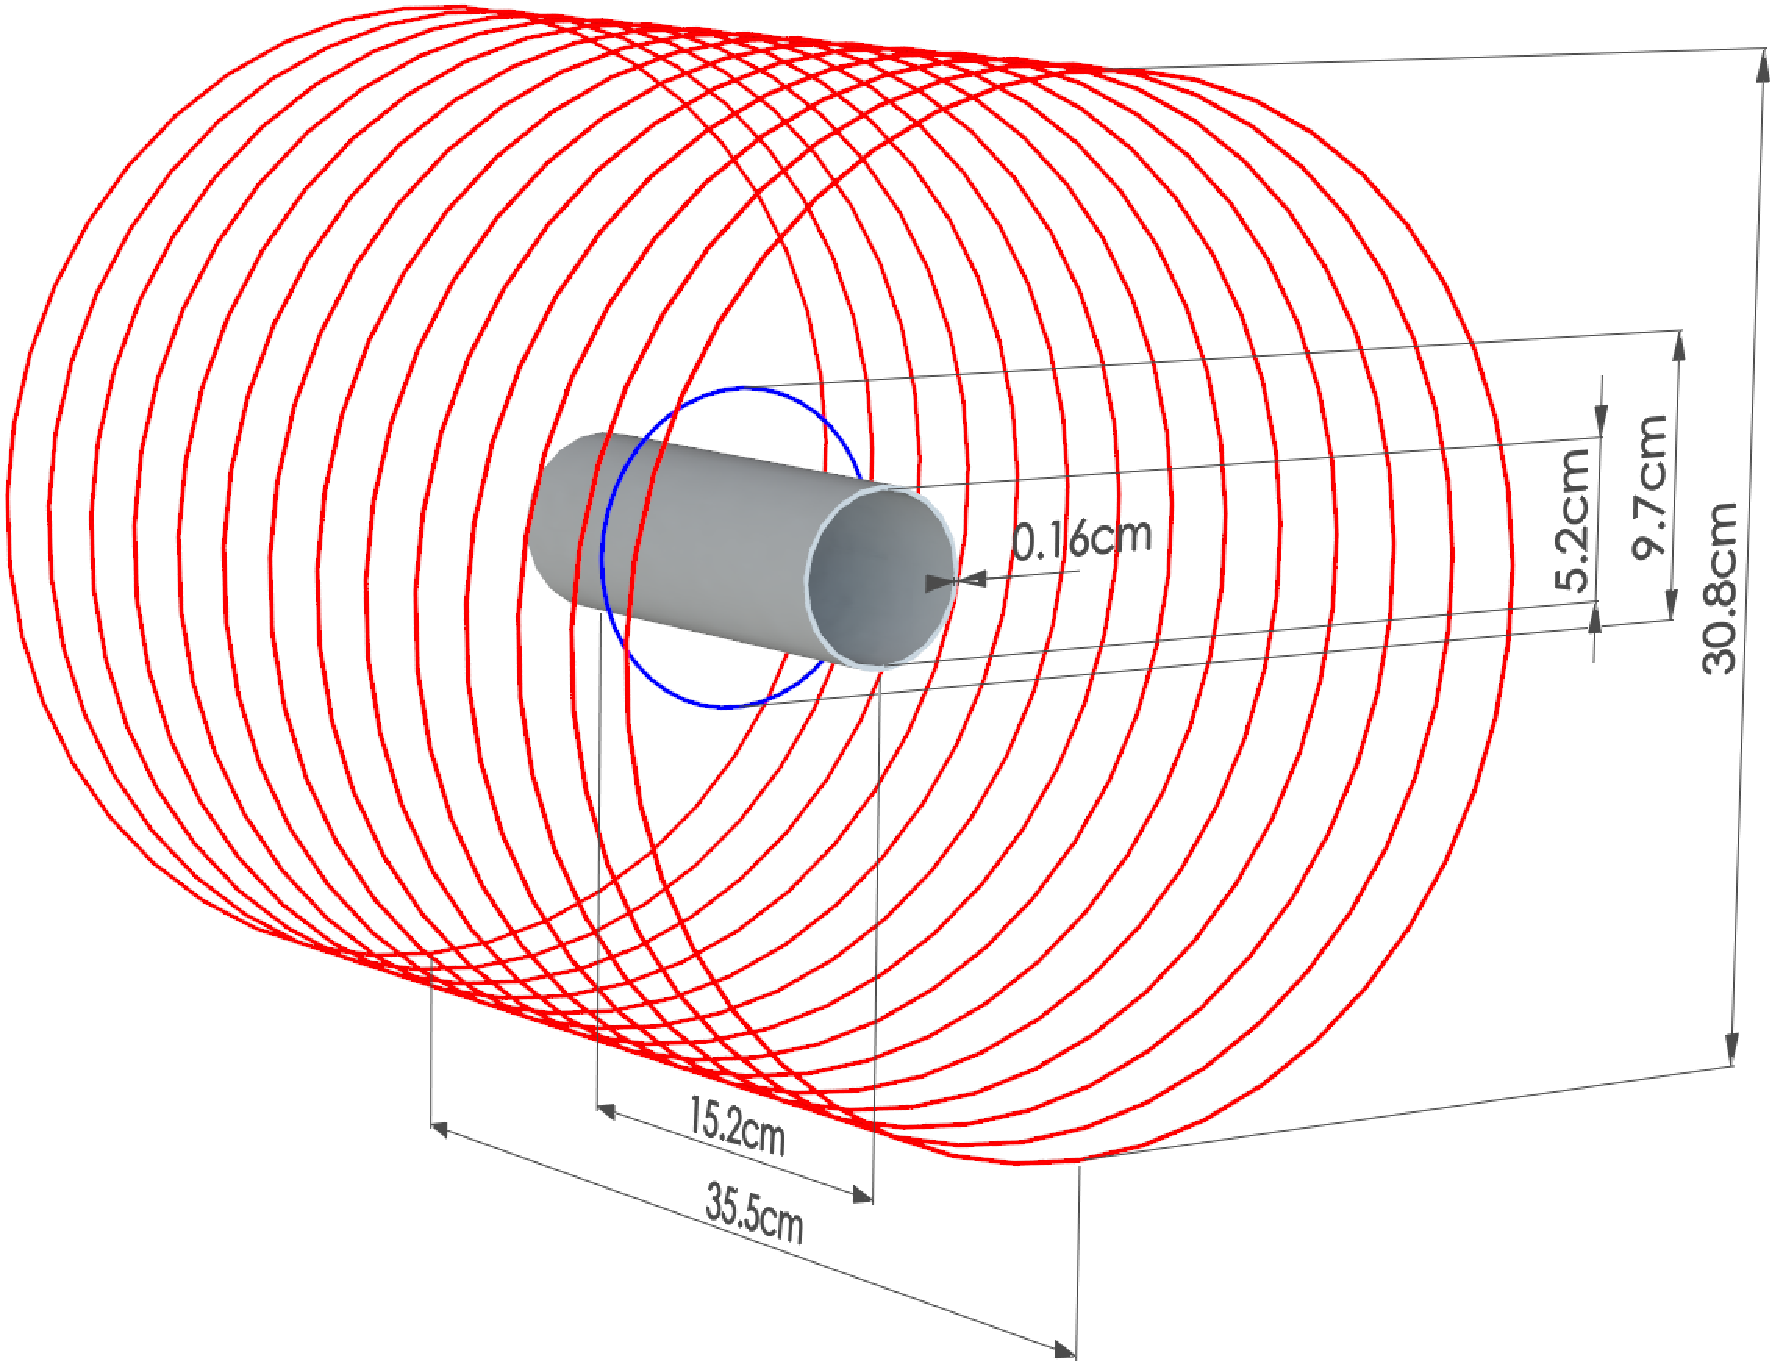
\includegraphics[width=0.7\textwidth]{to_jeff_new4.pdf}
    \caption[Drawing of the axial shielding factor measurement setup
    ]{(color online) Axial shielding factor measurement setup. The
      witness cylinder with an inner diameter of 5.2~cm and a length
      of 15.2~cm is placed inside a solenoid (shown in red) with a
      diameter of 30.8~cm and a length of 35.5~cm, containing 14
      turns.  The thickness of the witness cylinder is
      $1/16''=0.16$~cm.  The loop coil (shown in blue) is mechanically
      coupled to the witness cylinder and has a diameter of 9.7~cm.}
    \label{fig:geometry}
  \end{center}
\end{figure}

As shall be described in Section~\ref{sec:axialsyst}, a concern in the
measurement was changes in the field measured by the fluxgate that
could arise due to motion of the system components, or other
temperature dependences. This could generate a false slope with
temperature that might incorrectly be interpreted as a change in the
magnetic properties of the witness cylinder.

To address possible motion of the witness cylinder with respect to the
field generation system, another coil (the loop coil, also shown in
Fig.~\ref{fig:geometry}) was wound on a plastic holder mounted rigidly
to the witness cylinder.  The coil was one loop of copper wire with a
diameter of 9.7~cm.  Plastic set screws in the holder fixed the loop
coil to be coaxial with the witness cylinder.

Systematic differences in the results from the two coils (the
solenoidal coil, and the loop coil) were used to search for motion
artifacts.  As well, some differences could arise due to the different
magnetic field produced by each coil, and so such measurements could
reveal a dependence on the profile of the applied magnetic field.
This is described further in Section~\ref{sec:axialsyst}.

The temperature of the witness cylinder was measured by attaching four
thermocouples at different points along the outside of the cylinder.
This allowed us to observe the temperature gradient along the witness
cylinder.  To reduce any potential magnetic contamination, T-type
thermocouples were used, which have copper and constantan conductors.
(K-type thermocouples are magnetic.)

Thermocouple readings were recorded by a National Instruments NI-9211
temperature input module.  The magnetic field (signified by the
lock-in amplifier readout) and the temperature were recorded at a rate
of 0.2~Hz.

Temperature variations in the experiment were driven by ambient
temperature changes in the room, although forced air and other
techniques were also tested.  These are described further in
Section~\ref{sec:axialsyst}.


\subsubsection{Data and Interpretation\label{sec:axialsyst}}

An example of the typical data acquired is shown in
Fig.~\ref{fig:B_vs_Temp}.  For these data, the field applied by the
solenoid coil was 1~$\mu$T in amplitude, at a frequency of 1~Hz.
Fig.~\ref{fig:B_vs_Temp}(a) shows the temperature of the witness
cylinder over a 70-hr measurement.  The temperature changes of 1.4~K
are caused by diurnal variations in the laboratory.  The shielded
magnetic field amplitude $B_s$ within the witness cylinder is
anti-correlated with the temperature trend as shown in
Fig.~\ref{fig:B_vs_Temp}(b).  Here, $B_s$ is the sum in quadrature of
the amplitudes of the in-phase and out-of-phase components (most of
the signal is in phase).  The magnetic field is interpreted to depend
on temperature, and the two quantities are graphed as a function of
one another in Fig.~\ref{fig:B_vs_Temp}(c).  The slope in
Fig.~\ref{fig:B_vs_Temp}(c) has been calculated using a linear fit to
the data.  The relative slope at 23$^\circ$C was found to be
$\frac{1}{B_s}\frac{dB_s}{dT}=-0.75\%$/K.

\begin{figure}
  \begin{center}
    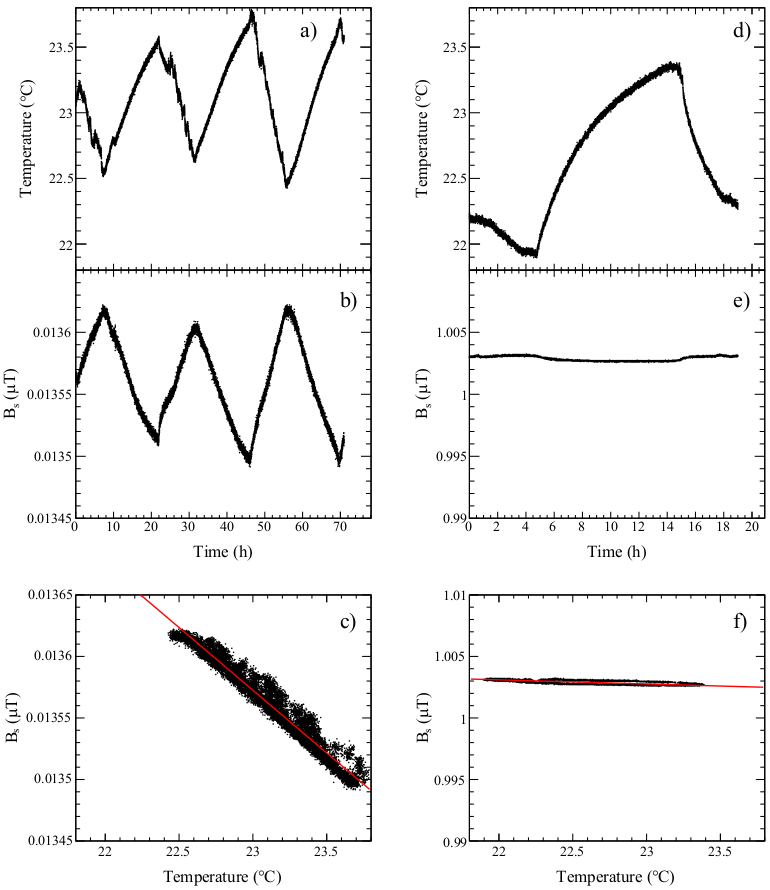
\includegraphics[width=\textwidth]{fig3.png}
    \caption[Ambient temperature and shielded magnetic field amplitude
    measurement]{Ambient temperature and shielded magnetic field
      amplitude, measured over a 70 hour period. (a) temperature of
      the witness cylinder as a function of time.  (b) magnetic field
      amplitude measured by fluxgate at center of witness cylinder
      vs.~time.  (c) magnetic field vs.~temperature with linear fit to
      data giving $\frac{1}{B_s}\frac{dB_s}{dT}=-0.75\%$/K (evaluated
      at 23$^\circ$C).  In panels (d), (e), and (f), the same
      quantities are shown for a 20-hour run with a copper cylinder in
      place of the witness cylinder with the linear fit giving
      $\frac{1}{B_s}\frac{dB_s}{dT}=-0.03\%$/K.}
    \label{fig:B_vs_Temp}
  \end{center}
\end{figure} 

Figs.~\ref{fig:B_vs_Temp}(d), (e), and (f) show the same measurement
with essentially the same settings, when the mu-metal witness cylinder
is replaced by a copper cylinder.  A similar relative vertical scale
has been used in Figs.~\ref{fig:B_vs_Temp}(e) and (f) as
Figs.~\ref{fig:B_vs_Temp}(b) and (c).  This helps to emphasize the
considerably smaller relative slope derived from panel (f) compared to
panel (c).  A variety of measurements of this sort were carried out
multiple times for different parameters such as coil current.  Running
the coil at the same current tests for effects due to heating of the
coil, whereas running the coil at a current which equalizes the
fluxgate signal to its value when the mu-metal witness cylinder is
present tests for possible effects related to the fluxgate.  For all
measurements the temperature dependence of the demodulated magnetic
signal was $<0.1$\%/K, giving confidence that unknown systematic
effects contribute below this level.

Some deviations from the linear variation of $B_s$ with $T$ can be
seen in the data, particularly in Figs.~\ref{fig:B_vs_Temp}(a), (b),
and (c).  For example, when the temperature changes rapidly, the
magnetic field takes some time to respond, resulting in a slope in
$B_s-T$ space that is temporarily different than when the temperature
is slowly varying.  This is typical of the data that we acquired, that
the data would generally follow a straight line if the temperature
followed a slow and smooth dependence with time, but the data would
not be linear if the temperature varied rapidly or non-monotonically
with time.  We also tried other methods of temperature control, such
as forced air, liquid flowing through tubing, and thermo-electric
coolers.  The diurnal cycle driven by the building's air conditioning
system gave the most stable method of control and the most
reproducible results for temperature slopes.

As mentioned earlier, data were acquired for both the solenoid coil
and the loop coil. A summary of the data is provided in
Table~\ref{tab:axial}.  Repeated measurements of temperature slopes
using the loop coil fell in the range
0.4\%/K~$<\vert\frac{1}{B_s}\frac{dB_s}{dT}\vert<$~1.5\%/K.  Similar
measurements for the solenoidal coil yielded
0.3\%/K~$<\vert\frac{1}{B_s}\frac{dB_s}{dT}\vert<$~0.8\%/K.

\begin{table}
\begin{center}
\begin{tabular}{cccc}\hline
Trial & $\frac{1}{B_s}\frac{dB_s}{dT}$ & Coil \\
\#    & (\%/K) & type \\\hline
 1 & -0.32 & solenoid \\
 2 & -0.30 & solenoid \\
 3 & -0.33 & solenoid \\
 4 & -1.53 & loop \\
 5 & -0.42 & loop \\
 6 & -1.30 & loop \\
 7 & -0.74 & solenoid \\
 8 & -1.05 & loop \\
 9 & -0.73 & solenoid \\
10 & -1.23 & loop \\
11 & -0.75 & solenoid \\
12 & -1.12 & loop \\\hline
\end{tabular}
\caption[Summary of the AC axial shielding factor
measurements]{Summary of data acquired for the AC axial shielding
  factor measurements, in chronological order.  Data with an applied
  field of $\sim 1-6\mu T$ and a measurement frequency of 1~Hz are
  included.  Data which used daily fluctuations of the temperature
  from 21-24$^\circ$C over a 10-80 hour period are included.  Other
  data acquired for systematic studies are not included in the
  table.\label{tab:axial}}
\end{center}
\end{table}

In general, the slopes measured with the loop coil were larger than
for the solenoidal coil.  This is particularly evident for
measurements 6-12, which were acquired daily over the course of a few
weeks alternating between excitation coils but all used the same
witness cylinder and otherwise without disturbing the measurement
apparatus.  A partial explanation of this difference is offered by the
field profile generated by each coil, and its interaction with the
witness cylinder.  This is addressed further in
Section~\ref{sec:axialsims}.

The other difference between the loop coil and the solenoidal coil was
that the loop coil was rigidly mounted to the witness cylinder,
reducing the possibility of artifacts from relative motion.  Given
that this did not reduce the range of the measured temperature slopes
we conclude that relative motion was well controlled in both cases.

Several other possible systematic effects were considered, all of
which were found to give uncertainties on the measured slopes
$<0.1\%$/K.  These included: thermal expansion of components including
the witness cylinder itself, temperature variations of the magnetic
shielding system within which the experiments were conducted,
degaussing of the witness cylinder, and temperature slopes of various
components e.g. the fluxgate magnetometer and the lock-in amplifier.

%%% null meast
As mentioned earlier in reference to Fig.~\ref{fig:B_vs_Temp}(d), (e),
and (f), the stability of the system was also tested by replacing the
mu-metal witness cylinder with a copper cylinder and in all cases
temperature slopes $<0.1$\%/K were measured, giving confidence that
other unknown systematic effects contribute below this level.

Based on the systematic effects that we studied, we conclude that they
do not explain the ranges of values measured for
$\frac{1}{B_s}\frac{dB_s}{dT}$.  We suspect that the range measured is
either some yet uncharacterized systematic effect, or a complicated
property of the material. We use this range to set a limit on the
slope of $\mu(T)$


\subsubsection{Geometry correction and determination of $\mu(T)$\label{sec:axialsims}}

To relate the data on $B_s(T)$ to $\mu(T)$, the shielding factor of
the witness cylinder as a function of $\mu$ must be known. Finite
element simulations in FEMM and OPERA were performed to determine this
factor.  The simulations are also useful for determining the effective
values of $B_m$ and $H_m$ in the material, which will be useful to
compare to the case for typical nEDM experiments when the innermost
shield is used as a flux return.

For closed objects, such as spherical
shells~\cite{bidinosti2014passive, urankar1996design}, the shielding
factor approaches infinity as $\mu \rightarrow \infty$, and
$\vert\frac{\mu}{B_s}\frac{dB_s}{d\mu}\vert\rightarrow 1$.  Because
the witness cylinders are open ended, the shielding factor
asymptotically approaches a constant rather than infinity in the
high-$\mu$ limit, and as a result
$\vert\frac{\mu}{B_s}\frac{dB_s}{d\mu}\vert<1$ here.  From the
simulations the ratio $\frac{\mu}{B_s}\frac{dB_s}{d\mu}$ was
calculated.  A linear model of the material was used where
$\bold{B_m}=\mu\bold{H_m}$ with $\mu$ constant.


The simulations differed slightly in their results, dependent on
whether OPERA or FEMM was used, and whether the solenoidal coil or
loop coil were used.  Based on the simulations, the result is
$\vert\frac{\mu}{B_s}\frac{dB_s}{d\mu}\vert=0.42-0.50$ for the
solenoidal coil, with the lower value being given by FEMM and the
upper value being given by a 3D OPERA simulation, for identical
geometries.  This is somewhat lower than the value suggested by
Ref.~\cite{paperno1999charts} with fits to simulations performed
in OPERA, which we estimate to be 0.6.  We adopt our value since it is
difficult to determine precisely from
Ref.~\cite{paperno1999charts}.  For the loop coil, we determine
$\vert\frac{\mu}{B_s}\frac{dB_s}{d\mu}\vert=0.56-0.65$, the range
being given again by a difference between FEMM and OPERA.

Combining the measurement and the simulations, the temperature
dependence of the effective $\mu$ (at $\mu_r=20,000$ which is
consistent with our measurements) can be calculated by
equation~(\ref{eqn:axial}).  The results of the simulations and
measurements are presented in Table~\ref{tab:axialsummary}. Combining
the loop coil and solenoidal coil results, we find
0.6\%/K~$<\frac{1}{\mu}\frac{d\mu}{dT}<2.7\%$/K to represent the full
range for the possible temperature slope of $\mu$ that observed in
these measurements.

\begin{table}
\begin{center}
\begin{tabular}{|c|c|c|c|}
\hline 
  & $\vert \frac{\mu}{B_s}\frac{dB_s}{d\mu}\vert$ & $\vert \frac{1}{B_s} \frac{dB_s}{dT}\vert$~(\%/K) & $\frac{1}{\mu}\frac{d\mu}{dT}$~(\%/K) \\ 
 & (simulated) & (measured) & (extracted) \\
\hline 
Solenoidal Coil & 0.42-0.50 & 0.3-0.8 & 0.6-1.9 \\ 
\hline 
Loop Coil & 0.56-0.65 & 0.4-1.5 & 0.6-2.7 \\ 
\hline 
\end{tabular} 
\caption[Summary of finite element simulations and shielding factor
measurements]{Summary of OPERA and FEMM simulations and shielding
  factor measurements, resulting in extracted temperature slopes of
  $\mu$.}
\label{tab:axialsummary}
\end{center}

\end{table}


As stated earlier, the simulations also provided a way to determine
the typical $B_m$ and $H_m$ internal to the material of the witness
cylinder.  According to the simulations, the $B_m$ amplitude was
typically 100~$\mu$T and the $H_m$ amplitude was typically 0.004~A/m.
These are comparable to the values normally encountered in nEDM
experiments, recalling from Section~\ref{sec:calculation} that
$H_m<0.007$~A/m for the innermost magnetic shield of an nEDM
experiment.  A caveat is that these measurements were typically
conducted using AC fields at 1~Hz, as opposed to the DC fields
normally used in nEDM experiments.
